\documentclass[a4paper, 11pt]{report}
\usepackage{graphicx}
\usepackage{xspace}
\usepackage[margin= 1in,includefoot]{geometry}
\newcommand\nth{\textsuperscript{th}\xspace}
\usepackage{xcolor}
\usepackage{lipsum}
\usepackage{listings}
\usepackage{amssymb} %maths
\usepackage{amsmath} %maths
\usepackage{mathptmx}
\begin{document}
\begin{figure}

\includegraphics[scale=.63]{medipol.png}
\centering
\end{figure}
\begin{titlepage}
\title{Introduction to Computer Engineering \\ Fall 2021, Assignment 1}
\author{by 64160010 - Rumeysa ÇELİK, Istanbul Medipol University}
\date{Due on Saturday October $23^{th}$, 2021 by 18:00 PM}
\maketitle
\end{titlepage}
{\center{\section*{{\textbf{Parameters Specific To Your Submission}}}}}
{\setlength{\parindent}{0pt}{In this assignment we will use the digits from your IDs. We define the following numbers
which are the \textbf{same} as the \textbf{numbers} you used in your assignment :}
\\ \\
$c_1$: The average of of digits from your student ID, \textbf{rounded} + 1. Use Excel file provided
to determine $c_1$.
\\ \\ My student ID is: 64160010
\begin{align*}
Average : \frac{6+4+1+6+0+0+1+0}{8} = \frac{18}{8} = 2.25 \approx 2 \\
c_1 = 2
\end{align*}
\\
$c_2$ : The average of digits from your Turkish ID, \textbf{rounded} + 1. Use the Excel file to determine $c_2$.
\\ \\
My Turkish ID is: 33098186424
\begin{align*}
Average: \frac{3+3+0+9+8+1+8+6+4+2+4}{11} = \frac{48}{11} = 4.36363636 \approx 4 \\
c_2 = 4
\end{align*}
\\
$c_3$: If $(c_1 \geq c_2)$ then $c_3 = 1$ otherwise $c_3 = -1$ .
\\ \\
$c_1 < c_2$ so that by $c_3 = -1$.
\\ \\
$c_4$ = $c_1$ + $c_2$.
\\ \\
Then,
\begin{align*}
c_4 = 2 + 4 = 6\\
c_4 = 6
\end{align*}
\\
$c_5$ : The first digit for your student ID.
\\ \\
My Student ID is: 64160010
\\ So that by $c_5$ = 6
\newpage
\section*{\textbf{Question 1 (40 points): Monitoring Covid Patients in Quarantine}}

The government of Turkey wants to develop a Bluetooth based system in order to track
Covid patients under quarantine:
\begin{enumerate}
\item Every Covid patient will wear a bracelet with active Bluetooth connectivity. The
Bluetooth devices have their own unique MAC address when they try to connect to
another Bluetooth receiver.
\item The bracelet continuously sends an Alive message to a government server via connection
either via a phone or another Internet connected Bluetooth device.
\item If the bracelet is cut, the Bluetooth stops working.
\item If the government server does not receive Alive message for any reason, it will initiate
a call and a search for the patient.
\item Locations such as malls, buses, and government office entrances are equipped with a
Bluetooth transceiver to get Bluetooth signals from nearby devices. If a patient runs
away from his/her quarantine period, then at these locations he/she can be caught via
the identification of the MAC address.
\end{enumerate}
\textbf{By making as many reasonable assumptions as you can wish}, provide details for the
following items:
\begin{enumerate}
\item[a.] (10 pts.) The key functional blocks of your proposed design. This will show the main
blocks and their connection with each other. This is not a flowchart.
\\ \\
{\color{blue}{There is no unique approach here. However, most of the main blocks given in Figure 1 are expected.}}
\item[b.] (10 pts.) How would you apply abstraction for your blocks. Provide details in 1-3 sentences for each block.
\\ \\
{\color{blue}{Each subblock is abstracted with minimal data transfer and the internal processing of each block is encapsulated. The following abstraction can be applied for each module. You can view Figure 1 below.}}
\begin{figure}[h]
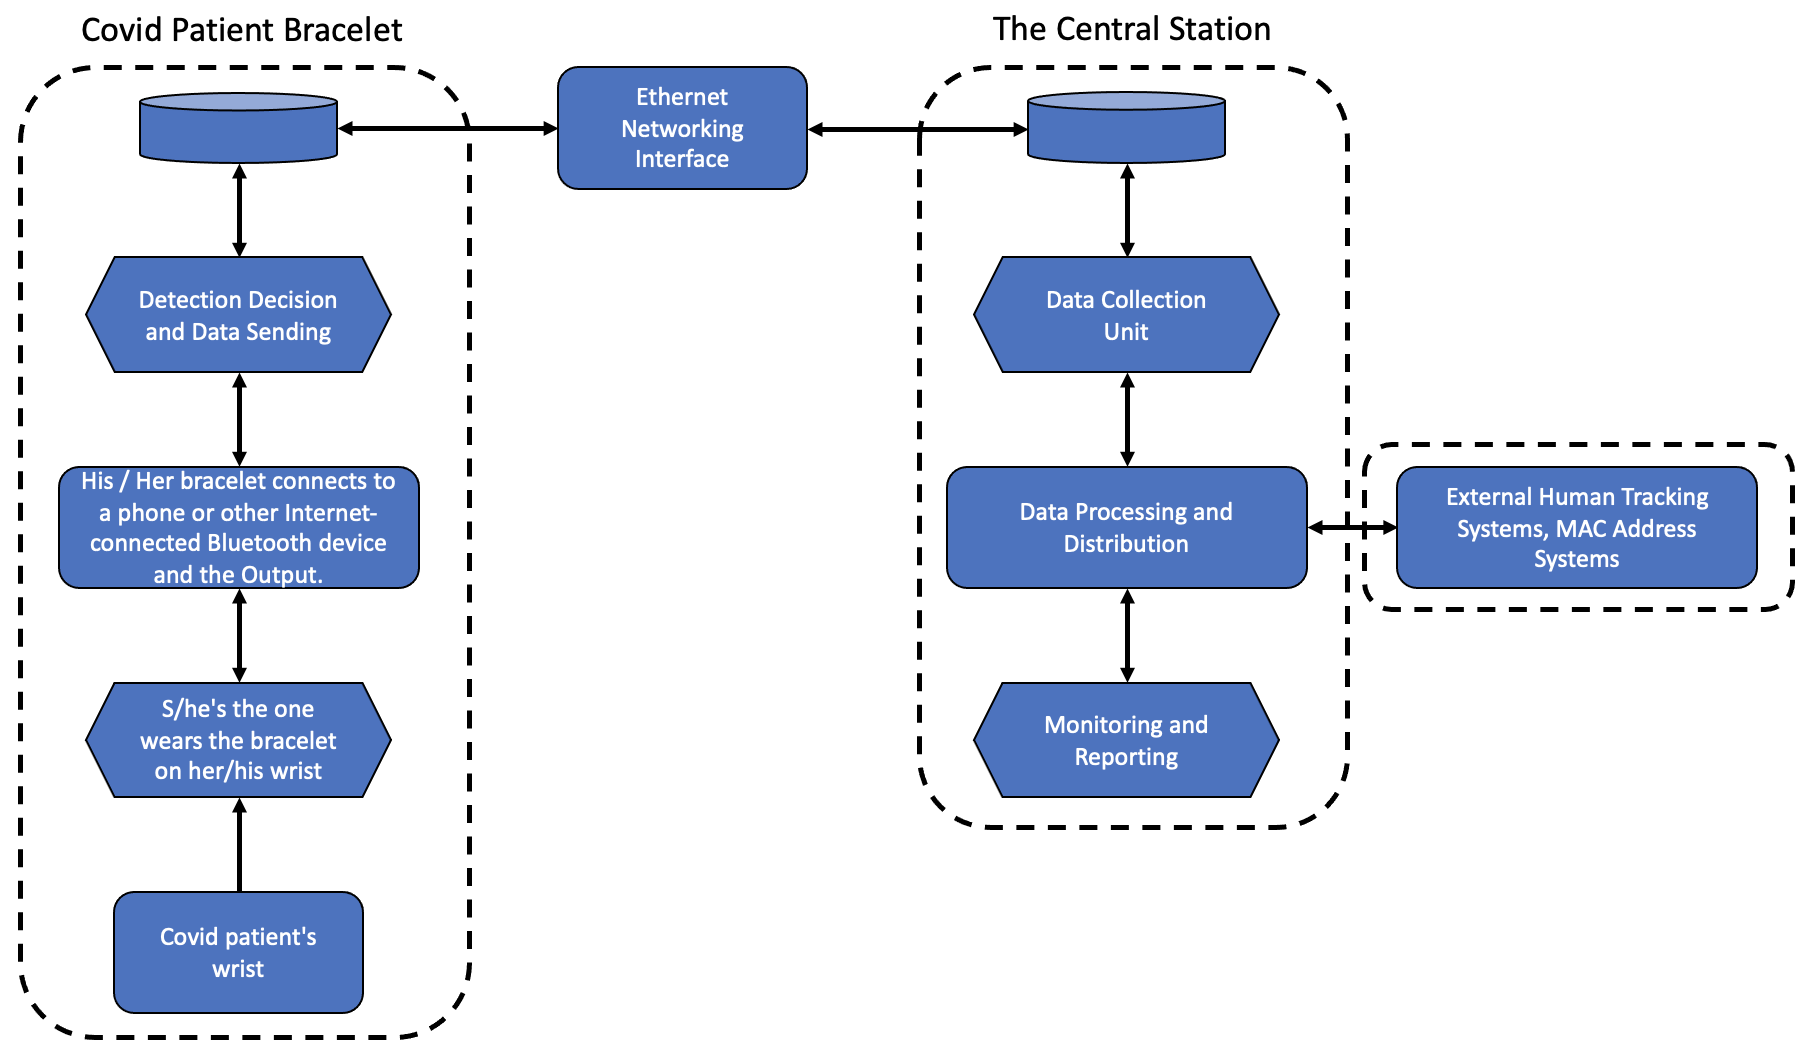
\includegraphics[scale=.33]{1.png}
\centering
\caption{Main functional blocks.}
\end{figure}
\newpage
\begin{enumerate}
{\color{blue}{\item[(a)] Covid patient's wrist: A person with Covid-19 needs their wrist to wear the bracelet.
\item[(b)] S/he's the one wears the bracelet on her/his wrist: Covid patient wears bracelet.
\item[(c)] His / Her bracelet connects to a phone or other Internet-connected Bluetooth device and the Output: The bracelet Covid patient continuously sends a Live message to a government server via connection via a phone or other Internet-connected Bluetooth device. Bluetooth will stop working if the bracelet is cut off. If the state server does not receive a live message for any reason, it initiates a call and calls the patient.
\item[(d)] Detection  Decision  and  Data  Sending: Only the MAC address is visible and this information is sent to a central station over the internet. Only input is provided for the detection value and an Ethernet output is provided for sending data. All processing and data preparation for sending is hidden inside this block. From the outside, it only sees two input/output ports: one for input data and one for output data over Ethernet.
\item[(e)] Data Collection Unit: Only two Ethernet interfaces are Provided here: to receive data and to send to Data processing centre. Some data definitions are made within this unit, but this process is hidden.
\item[(f)] Data Processing and Distribution: Again, only Ethernet interface is provided for communication with Data Collection Unit, Tracking Systems, Monitoring and Reporting servers. Many operations are performed within this unit, but all operations are hidden. Only one Ethernet connection is visible from the outside.
\item[(g)] Monitoring and Reporting: Data is collected and presented either as graphs or maps. All transactions are hidden. The connection will be via Ethernet.
\item[(h)] Tracking  Systems: An Ethernet interface to MAC addresses to retrieve users' information. All communication details are hidden, but an Ethernet interface is provided for communication.}}
\end{enumerate}
\item[c.] (5 pts.) How would you make your design modular?
\\ \\
{\color{blue}{By specifying standard interfaces for each block and separating the different functions, and then implementing them in a separate block. The diagram given in Figure 1 has a modular design. As explained in the previous section, for most of the blocks we would use an Ethernet interface and connect different modules. As can be seen, modules can be easily reused by other designs. We apply two modules for the corona patient wristband device: corona patients put this bracelet on their wrist and do not remove it.}}
\item[d.] (5 pts.) How would you apply standardization? \\ \\
{\color{blue}{Standardization is applied so that any module or block developed can be reused by another project. Here is a typical standardization list for each block diagram.}}
\begin{enumerate}
{\color{blue}{\item[(a)] Covid patient's wrist: A standard bracelet will be used to be worn on the wrist of Covid patients. Length and thickness will be standard based on body indexes.
\item[(b)] S/he's the one wears the bracelet on her/his wrist: A standard bracelet will be used to be worn on the wrist of Covid patients. Length and thickness will be standard based on body indexes.
\item[(c)] His / Her bracelet connects to a phone or other Internet-connected Bluetooth device and the Output: A simple enclosure for bracelets that allows to follow current Corona Virus patients so that bracelets can be used in standard typings. However, patients' wrist sizes may be different.
\item[(d)] Detection  Decision  and  Data  Sending: The standard Ethernet interface is used. Also, one of the simple data transfer protocols and encapsulation can be used so that there is no need to reinvent a data sending mechanism.
\item[(e)] Data Collection Unit:  Same as the previous part.
\item[(f)] Data  Processing  and  Distribution: It is necessary to ensure that the data distribution follows a typical practice for data distribution used in networking. It is preferable to use an Ethernet interface for easy integration.
\item[(g)] Monitoring and Reporting: One of the simple open source reporting tools is used. Microsoft tools can also be used for reporting. As for the reporting format, Maps by Google or other companies can be used.
\item[(h)] Tracking Systems: An Ethernet interface to the cellular operators to get the info of the users.}}
\end{enumerate}
\item[e.] (10 pts.) Develop an algorithm on how to catch patients breaking out their quarantine. Demonstrate this via a flowchart diagram.
\begin{figure}[h]
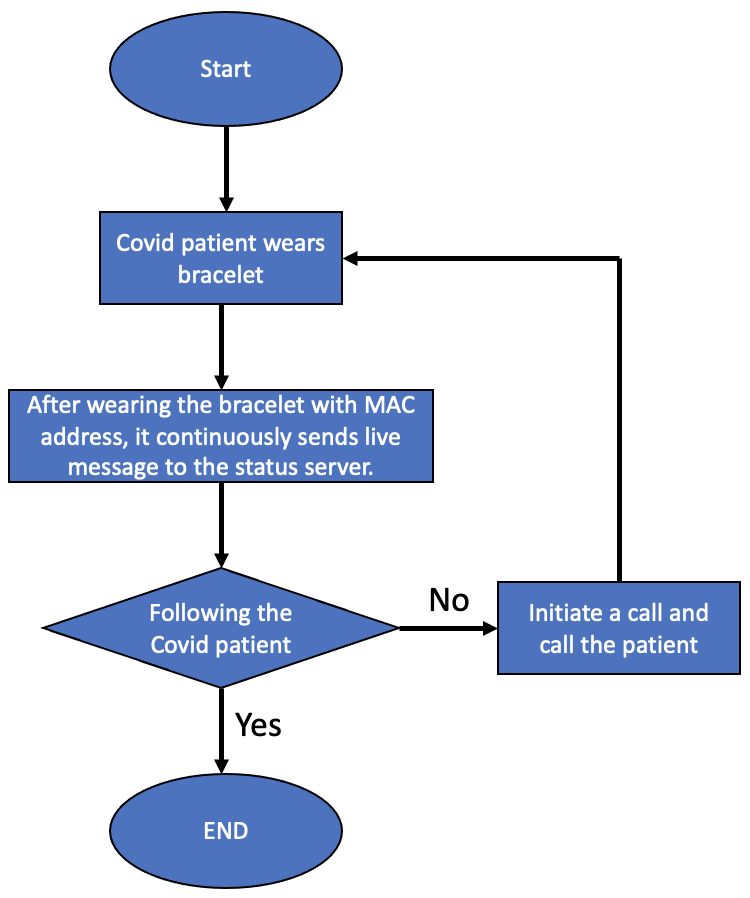
\includegraphics[scale=.33]{2.png}
\centering
\caption{Flowchart Diagram}
\end{figure}
\end{enumerate}

\section*{\textbf{Question 2 (30 points): Monitoring Covid Patients in Quarantine - The Overall System}}

For the system given in the first question, we want you to investigate the following items.
\begin{enumerate}
\item[a.] (20 pts.) Apply the the design process steps to the system given in Question 1. You can perform some research for the evaluation and analysis stages as if you are doing the research. Please explain each step in 1-3 sentences.
\\ \\
{\color{blue}{The design process steps are given below. For each step, a set of necessary actions needs to be performed.}}
\begin{enumerate}
{\color{blue}{\item[(a)] Recognizing  the  need  for  a  product  or  a  service: Currently, there are many people out there who pose a great risk by not quarantining themselves even though they have the virus. If these covid patients can be followed through bracelets, the spread of the virus can be reduced. Wearing these bracelets by Covid patients will make it easier to follow them, and thus the rate of spread of the virus will be greatly reduced.
\item[(b)] Problem definition and understanding: Current covid patient tracking is only available to the public through apps like "Life Fits Home". Moreover, since manual data entry is required, many do not enter data into the government system. The MAC address bracelets to be developed will continuously send a live message to a government server via connection via a phone or other Bluetooth device connected to the Internet.
\item[(c)] Research and preparation: Research needs to be done on how to follow Corona patients quickly, that is, how to follow a covid patient who is on the run within minutes. How this can be achieved needs to be determined. In addition, a software architecture that can report data to different state stations needs to be developed in order to catch carriers. More research can be done on how to make this situation easier so that it doesn't become a tedious task for humans.
\item[(d)] Conceptualization: Here's how each piece fits together. The patient with Covid will wear the Mac address bracelet and connect to a phone or other Internet-connected Bluetooth device. There will be a signal-based module that monitors whether the patient with Covid is in quarantine, an electronic reader that reads the output of the bracelet detector, and an electronic subsystem that sends this reading to the government central station.
\item[(e)] Synthesis: Since the bracelet has electronics, tests will need to be done on the computer. The ultimate goal is to see if the overall integrated system works the way we want to develop it.
\item[(f)] Evaluation: Its overall system will be designed and then checked for known conditions. Here, it will be evaluated whether the device detects correctly. In addition, it will be tested whether the MAC address information from the bracelet is transmitted to the central station correctly.
\item[(g)] Optimization: Based on the evaluation carried out in the previous step, changes will be made to the existing design. Multiple iterations of the design can be performed until the designed system meets the targeted performance.
\item[(h)] Presentation: A complete presentation will be prepared that includes the overall project description, benefits, ease of use and easy integration for a specific location. The presentation will also include videos on using the device. Finally, the presentation may also include a live demo of whether the bracelet is accurately tracking a patient with covid.}}
\end{enumerate}
\item[b.] (5 pts.) How would you set up your team for this project? Explain in terms of technical background as well as people’s personality.
\\ \\
{\color{blue}{The following team members can be used:\\ \\
Computer Engineers : For the software part required for communication with the central station, providing data to government systems and software interfaces.\\
Electrical Engineers: To design and operate the Signal system. Sending and receiving data with government servers.\\
Mechanical Engineers: Designing the mechanical part of the system for an easy-to-use wristband.\\ \\
The list can be expanded as long as justification is provided.}}
\item[c.] (5 pts.)  How would you protect your design?  Also provide a Trademark for your product.
\\ \\
{\color{blue}{Ideas can be protected in several ways:}}
\begin{enumerate}
{\color{blue}{\item[(a)] A patent is required for the overall system design.
\item[(b)] A patent is required for the tracking system.
\item[(c)] A utility patent is required for the appearance of the bracelet.
\item[(d)] A trademark is required.
\item[(e)] A service mark may even be provided.}}
\end{enumerate}
\end{enumerate}

\section*{\textbf{Question 3 (30 points): Development of Mathematical Models}}

For each of the following cases, develop a mathematical model for the testing in computer environments. You can make assumptions as needed.
\begin{figure}[h]
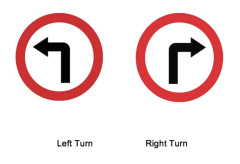
\includegraphics[scale=.53]{3.png}
\centering
\caption{Left and Right Turn Signs.}
\end{figure}
\begin{enumerate}
\item[a.] (10 pts.) You want to identify the Left and Right Signs given in Project Description file. These signs are also given in Fig. 1. One simple mathematical modelling would
be to count the red and white pixels and compare but then that would be the same for
both signs. Propose an alternative mathematical model that would differentiate these
two signs.
{\color{blue}{\begin{align*}
y = bx^{a/c}
\end{align*}}}
{\color{blue}{ a = Forward gear, c = reverse and b is the value of y when x = 1(it means to stop). If a/c $>$ 1,  then the direction is to the right. If the condition is the opposite, the direction is to the left.}}
\item[b.] (10 pts.) Assume that your autonomous car’s camera detects a Right Turn Signal $c_4$ meters away. We want you to turn right in a lane with width of $c_2$ meters. While you are turning your car, we want the passengers inside the car not feeling the centripetal acceleration for more than $c_1$ $m/s^2$. Provide a mathematical model for your autonomous car’s velocity. Please note that each student will have his/her own coefficients for the c values. Directly use the numerical values for your solution, not the expressions in terms of c coefficients.
{\color{blue}{\begin{align*}
y = bx^{a/c} \qquad b = 6 \quad a = 2 \quad c=2 \\
y = 6x^{2/2} \\
y = 6x
\end{align*}}}
\item[c.] (10 pts.) Assume that you are using a camera to ensure that you are on the center of
the lane. Your camera takes the picture of solid white line on the right side and the
yellow dashed line on the center of the road. It is assumed that you know the length
of dashed lines and the width of the yellow and white lines. Propose a mathematical
model on how you place your car in the center of the lane, assuming that you know
exactly where the cameras are placed in your autonomous car.
\end{enumerate}



























\end{document}